\documentclass[11pt]{article}
\usepackage{amsmath}

\usepackage{amstext}

\usepackage{amsthm}
\usepackage{color, fullpage, hyperref}
\usepackage{amssymb}
\usepackage{mathtools}
\usepackage{commath}

\usepackage{graphicx}
\usepackage{tikz, pgfplots, hf-tikz}
\pgfplotsset{compat=1.17}
\allowdisplaybreaks
\renewcommand\qedsymbol{$\blacksquare$}
\usepackage{tcolorbox}
\tcbuselibrary{theorems}
\tcbuselibrary{fitting}
\usepackage{empheq}

\usepackage[margin=0.5in, legalpaper]{geometry}
\usepackage{fancyvrb}

\newcommand{\R}{\mathbb{R}}
\newcommand{\qqlt}[1]{\qquad\leftarrow\text{#1}}
\newcommand{\question}[1]{$\displaystyle{#1}$}

\newcommand{\IBPreset}{\tcbset{
		colback=blue!25!purple!10!,
		colframe=blue!40,
		title= Aside: Integration by Parts
}}

\newcommand{\PFDpreset}{\tcbset{
		colback=blue!25!purple!10!,
		colframe=blue!20!purple!50!,
		title= Aside: Partial Fraction Decomposition
}}

\newcommand{\finaldef}[1]{
	\tcboxmath[colback=blue!25!purple!10!,
	colframe=red!40, notitle, center]{{#1}}
}

\DeclareMathOperator*{\di}{\mathrm{d}\!}
\def\at{
	\left.
	\vphantom{\int}
	\right|
}


\title{CSCB07 Midterm Notes}

%Put assignment number to suit.

\author{Vinesh Benny}

\date{\today}


\begin{document}

%\maketitle

\section{Version Control}

\begin{itemize}
	\item Two flavours of Version Control
		\begin{itemize}
			\item Centralized (B07 uses this)
			\item Decentralized
		\end{itemize}

	\item Centralised Version
		\begin{itemize}
			\item Keep code in a centralized location (the “Repository”)
			\item Code in repository is the ``Master Copy" (\textbf{\underline{Never}} directly modify)
			\item Instead make local copies of the repository on each computer you will be working on (working copy)
			\item When major changes are made to local copy that you want to save, ``commit" change to repo
			\item Tools allow you to revert to a previous version of the source code (only when commits have occurred)
		\end{itemize}

	\item Some Terminology

		\begin{minipage}[t][0.72in]{0.25\textwidth}
			\begin{itemize}
				\item Repository/Repo
				\item Client program
				\item Working copy
			\end{itemize}
		\end{minipage}
		\begin{minipage}[t]{0.4\textwidth}
			\begin{itemize}
				\item Checkout
				\item Commit
			\end{itemize}
		\end{minipage}


	\item Centralized systems include:
		\begin{itemize}
			\item \textbf{S}ub\textbf{V}ersio\textbf{n} (\textbf{SVN})
				\begin{itemize}
					\item SVN is the successor to \textbf{C}oncurrent \textbf{V}ersions \textbf{S}ystem (\textbf{CVS}), and was built to help fix many issues in CVS
				\end{itemize}
			\item Git
			\item Mercurial
			\item ClearCase
			\item Perforce
		\end{itemize}

	\item SSH and SCP are \textbf{not} version control systems
		\begin{itemize}
			\item \textbf{S}ecure \textbf{Sh}ell (SSH) is used to connect to a remote computer and work in a shell on that computer
			\item \textbf{S}ecure \textbf{C}o\textbf{p}y (SCP) is used to:
				\begin{itemize}
					\item Securely copy files from one computer to another
					\item Transfer a copy of the files but does \textbf{not} version them
				\end{itemize}
		\end{itemize}

	\item Version Control – Managing Concurrency

		\emph{When two or more people want to edit the same file at the same time}
			\begin{itemize}
				\item Pessimistic concurrency
					\begin{itemize}
						\item Only allow one writeable copy of each file
						\item e.g. Microsoft Visual SourceSafe, Rational ClearCase
					\end{itemize}

				\item Optimistic concurrency
					\begin{itemize}
						\item Allow writes, fix issues afterwards
						\item Merging
							\begin{itemize}
								\item SVN is either able to merge without help from the user, or
								\item \textit{Conflict}: SVN needs the user to resolve the conflict
							\end{itemize}
						\item e.g. Subversion, CVS, Perforce
					\end{itemize}
				\newpage
				\item Optimistic Concurrency – Merging Options

					Select from: \textbf{(p)} postpone, \textbf{(df)} diff-full, \textbf{(e)} edit, \textbf{(mc)} mine-conflict, \textbf{(tc)} theirs-conflict and \textbf{(s)} show all options.\\[-15pt]
					\begin{center}
						\begin{minipage}[c]{0.6\textwidth}
					\begin{itemize}
						\item[(e) edit] - changed merged file in an editor
						\item[(df) diff-full] - show all changes made to merged file4
						\item[(r) resolved]  - accept merged version of file\\
						\item[(dc) display-conflict] - show all conflicts (ignoring merged version)
						\item[(mc) mine-conflict] -  accept my version for all conflicts (same as above)
						\item[(tc) theirs-conflict] -  accept their version for all conflicts (same as above) \\
						\item[(mf) mine-full] - accept my version of entire file (even non-conflicts)
						\item[(tf) theirs-full]  - accept my version of entire file (same as above)\\
						\item[(p) postpone] - mark the conflict to be stored later
						\item[(l) launch] - launch external tool to resolve conflict
						\item[(s) show all] - show this list
					\end{itemize}
					\end{minipage}
					\end{center}
			\end{itemize}

	\item Integrating the code - Reasons for merge conflicts\\[-15pt]

		\begin{minipage}[t]{0.3\textwidth}
			\begin{itemize}
			\item Communication
			\item Complex code bases
			\item Experimental features being built
			\end{itemize}
		\end{minipage}
		\begin{minipage}[t]{0.5\textwidth}
			\begin{itemize}
				\item More than one project on the go that impacts this code
				\item Two features being built in same class by different developers
			\end{itemize}
		\end{minipage}

	\item Branching
		\begin{itemize}
			\item Branches are divergent copies of development lines
					\item These versions are used to build out complex features, or do experiments,
					without having an impact on the main code line
			\item Strategies include:
				\begin{itemize}
					\item No branching
					\item Release branching
					\item Feature branching
				\end{itemize}
		\end{itemize}

	\item Storage scheme
		\begin{itemize}
			\item Storing every copy of every file generated over the course of a project is not practical
			\item Version control systems store incremental differences in files/folder structures
			\item These differences store enough information to re-construct previous versions, without storing every single copy ever made of the file
		\end{itemize}

	\item What’s Stored Where
		\begin{itemize}
			\item Server side: out of scope
			\item Local copy contains a special directory, \textbf{.svn}
				\begin{itemize}
					\item It stores (locally) the information subversion needs to keep track of your files, version numbers, where the repository is, etc.
					\item Needless to say, you should not mess with the contents of this directory. Let subversion do its job
				\end{itemize}
		\end{itemize}

	\item General rules
		\begin{itemize}
			\item Update and commit frequently
			\item Never break the main branch
			\item Always comment clearly what changes are in a revision
			\item Test all code before accepting merge
			\item Communicate with your team!
		\end{itemize}
\end{itemize}

\newpage
\section{Introduction to Java}
\begin{itemize}

	\item What is Java?
		\begin{itemize}
			\item An object-oriented language invented by James Gosling in 1994 at Sun Microsystems
			\item Write once, run anywhere (WORA)
			\item Widely-used in industry
			\item Used to develop software running on:
%				\begin{itemize}
%					\item Desktop Computers
%					\item Servers
%					\item Mobile devices
%				\end{itemize}
				\begin{itemize}
				\begin{minipage}[t]{0.25\textwidth}
					\item Desktop Computers
				\end{minipage}
				\begin{minipage}[t]{0.15\textwidth}
					\item Servers
				\end{minipage}
				\begin{minipage}[t]{0.2\textwidth}
					\item Mobile devices
				\end{minipage}
				\end{itemize}
		\end{itemize}

	\item Java Programs
		\begin{enumerate}
			\item Writing the source code using a text editor
			\item Translating the source code into Java bytecode using a compiler
				\begin{itemize}
					\item Bytecode is similar to machine instructions but is architecture neutral and can run on any platform that has a Java Virtual Machine (JVM)
				\end{itemize}
			\item Executing the bytecode
				\begin{itemize}
					\item The JVM is an interpreter: it translates bytecode into the target machine language code one at a time rather than the whole program as a single unit
					\item Each step is executed immediately after it is translated\\[-21pt]
				\end{itemize}
		\end{enumerate}
	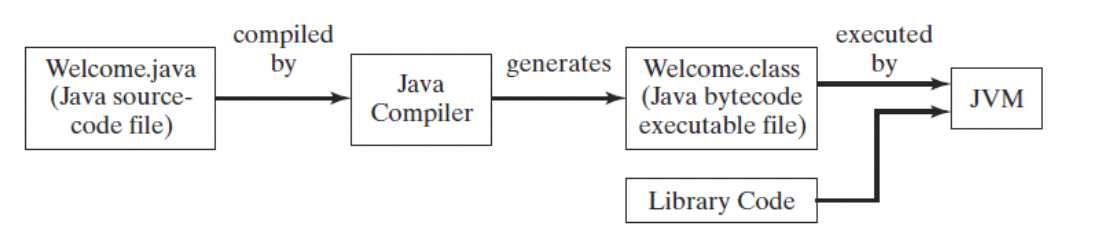
\includegraphics[scale=.75]{Compile flow.png}\\[-30pt]

	\item Integrated Development Environment
		\begin{itemize}
			\item A system comprising several tools that facilitate software development and testing
			\item Popular IDEs:
				\begin{itemize}
					\begin{minipage}[t]{0.15\textwidth}
						\item Eclipse
					\end{minipage}
					\begin{minipage}[t]{0.15\textwidth}
						\item NetBeans
					\end{minipage}
					\begin{minipage}[t]{0.2\textwidth}
						\item IntelliJ
					\end{minipage}
				\end{itemize}
		\end{itemize}

	\item Data Types
		\begin{itemize}
			\item Eight primitive types
				\begin{itemize}
					\item byte, char, short, int, long, float, double, boolean
				\end{itemize}
			\item Objects
				\begin{itemize}
					\item Defined using \textbf{classes}
					\item Java provides wrapper classes to use primitive types as objects (e.g. Integer, Double, etc)
				\end{itemize}
		\end{itemize}

	\item Numeric Primitive Types
%	\includegraphics[scale=.7]{Primitive types.png}
	\begin{center}
	\begin{tabular}{ l l l }
		\hline
		\textit{Name} & \textit{Range} & \textit{Storage Size}\\
		\hline\\[-10pt]
		\textbf{byte} & $ -2^7 $ to $ 2^7 - 1 \, (-128 \text{ to } 127)  $  & 8-bit signed\\
		\textbf{short} & $ -2^{15} $ to $ 2^{15} - 1 \, (-32768 \text{ to } 32767)  $ & 16-bit signed\\
		\textbf{int} & $ -2^{31} $ to $ 2^{31} - 1 \, (-2147483648 \text{ to } 2147483647)  $ & 32-bit signed\\
		\textbf{long} & $ -2^{63} $ to $ 2^{63} - 1  $ & 64-bit signed\\
		 & (i.e., $-9223372036854775808 \text{ to } 9223372036854775807$) & \\
		 \textbf{float} & Negative range: $ -3.4028235\text{E} + 38$ to $ -1.4\text{E} -45$ & 32-bit IEEE 754\\
		 & Positive range: $ 1.4\text{E} -45 $ to $ 3.4028235\text{E} + 38 $ & \\
		 \textbf{double} & Negative range: $ -1.7976931348623137\text{E} + 38$ to $ -4.9\text{E} - 324$ & 64-bit IEEE 754\\
		 & Positive range: $4.9\text{E} - 324$ to $1.7976931348623137\text{E} + 38$ &
		\end{tabular}
	\end{center}

	\item Classes
		\begin{itemize}
			\item A typical Java class includes the following:
				\begin{itemize}
					\item Data fields to represent the state of an object
					\item Methods to represent the behavior of an object. Each method has:
						\begin{itemize}
							\item A return type (\textbf{void} if nothing is returned)
							\item Zero or more arguments
						\end{itemize}
					\item Special type of methods, known as constructors, that perform initialization actions. A constructor:
						\begin{itemize}
							\item Has no return type (not even \textbf{void})
							\item Has zero or more arguments
							\item Should have the same name as the class
							\item Is invoked using the \textbf{new} operator
						\end{itemize}
				\end{itemize}
			\item Instantiation is creating an object (or an instance of a class)
		\end{itemize}

	\item The \textit{main} method
		\begin{itemize}
			\item The main method is the entry point where the program begins
			execution
			\item Should have the following form:
				\begin{Verbatim}
public static void main(String [] args) {
	//write your code here
}
				\end{Verbatim}
		\end{itemize}

	\item Default values
		\begin{itemize}
			\item The default value of a data field is:
			\begin{itemize}
				\begin{minipage}[t]{0.25\textwidth}
					\item \textbf{\textit{null}} for a reference type
				\end{minipage}
				\begin{minipage}[t]{0.25\textwidth}
					\item \textbf{0} for a numeric type
				\end{minipage}

				\begin{minipage}[t]{0.25\textwidth}
					\item \textbf{false} for a boolean type
				\end{minipage}
				\begin{minipage}[t]{0.25\textwidth}
					\item \textbf{'$\backslash$u0000'} for a char type
				\end{minipage}
			\end{itemize}
			\item Java assigns no default value to a local variable inside a method
		\end{itemize}

	\item Scope
		\begin{itemize}
			\item The scope of fields and methods is the entire class
			\item The scope of a local variable starts from its declaration until the end
			of the block that contains it
		\end{itemize}

	\item Differences between Variables of Primitive Types and Reference Types
		\begin{itemize}
			\item Every variable represents a memory location that holds a value
			\item For a variable of a primitive type, the value is of the primitive type
			\item For a variable of a reference type, the value is a reference to where an object is located (i.e. a pointer)
			\item When you assign one variable to another:
				\begin{itemize}
					\item For a variable of a primitive type, the real value of one variable is assigned to
					the other variable
					\item For a variable of a reference type, the reference of one variable is assigned to the other variable.
				\end{itemize}
		\end{itemize}

	\item The \textit{this} reference
		\begin{itemize}
			\item The \textbf{this} \textit{keyword} is the name of a reference that an object can use to
			refer to itself
			\item It can be used to reference the object’s instance members
		\end{itemize}

	\item The \textit{static} modifier
		\begin{itemize}
			\item Static fields/methods can be accessed from a reference variable or
			from their class name
			\item Non-static (or instance) fields/methods can only be accessed from a reference variable
		\end{itemize}

	\item Arrays
		\begin{itemize}
			\item An array is a data structure that represents a collection of the same types of data
			\item Once an array is created, its size is fixed
				\begin{itemize}
					\item e.g. \textbf{int [] A = new int[10];}
				\end{itemize}
			\item The size of an array A can be found using \textbf{A.length}
			\item When an array is created, its elements are assigned the default value
			\item Array elements could be initialized individually
				\begin{itemize}
					\item e.g. \textbf{A[0] = 5;}
				\end{itemize}
			\item Array initializer (combines declaration, creation, and initialization)
				\begin{itemize}
					\item e.g. \textbf{double[] myList = {1.9, 2.9, 3.4, 3.5};}
				\end{itemize}
		\end{itemize}

	\item Two-dimensional Arrays
		\begin{itemize}
			\item The syntax for declaring a two-dimensional array is:
				\begin{itemize}
					\item \textbf{elementType [][] arrayRefVar;} (e.g. \textbf{int[][] matrix;})
				\end{itemize}
			\item For a two-dimensional array A, \textbf{A.length} returns the number of rows
			\item Two-dimensional array examples:\\
				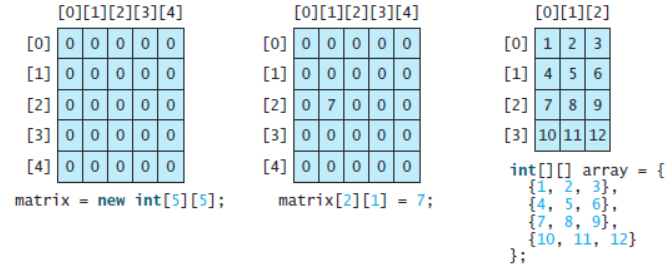
\includegraphics[scale=0.9]{array.png}
		\end{itemize}
\end{itemize}

\newpage

\section{Object Oriented Programming (1)}
\begin{itemize}
	\item Object-Oriented Thinking
		\begin{itemize}
			\item Procedural paradigm
				\begin{itemize}
					\item Focuses on designing methods
					\item Data and operations on the data are separate
				\end{itemize}
			\item Object-oriented paradigm
				\begin{itemize}
					\item Couples methods and data together into objects
					\item Organizes programs in a way that mirrors the real world
					\item A program can be viewed as a collection of cooperating objects
					\item Makes programs easier to develop and maintain
					\item Improves software reusability
				\end{itemize}
		\end{itemize}

	\item Inheritance
		\begin{itemize}
			\item Powerful feature for reusing software
			\item Helps avoid redundancy
			\item Different objects might have common properties and behaviors
				\begin{itemize}
					\item e.g. Person, Employee
				\end{itemize}
			\item Inheritance allows developers to
				\begin{itemize}
					\item Define a general class (or superclass). E.g. Person
					\item Extend the general class to a specialized class (or subclass). e.g. Employee
				\end{itemize}
			\item In Java, the keyword extends is used to indicate inheritance
		\end{itemize}

	\item Casting objects and the \textit{\textbf{instanceof}} operator
		\begin{itemize}
			\item It is always possible to cast an instance of a subclass to a variable of a superclass (known as upcasting)
				\begin{itemize}
					\item e.g. \textbf{Person p = new Employee();}
				\end{itemize}
			\item When casting an instance of a superclass to a variable of its subclass (known as \textit{downcasting}), explicit casting must be used
				\begin{itemize}
					\item e.g. \textbf{Person p = new Employee(); Employee e = (Employee)p;}
					\item If the superclass object is not an instance of the subclass, a runtime error occurs
					\item  It is a good practice to ensure that the object is an instance of another object before attempting a casting. This can be accomplished by using the \textit{\textbf{instanceof}} operator
				\end{itemize}
			\item Cating an object reference does not create a new object
		\end{itemize}

	\item Overloading and Overriding
		\begin{itemize}
			\item Overloading
				\begin{itemize}
					\item Defining methods having the same name but different signatures
						\begin{itemize}
							\item Signature: method name + types of its formal parameters
						\end{itemize}
					\item Overloading methods can make programs clearer and more readable
				\end{itemize}
			\item Overriding
				\begin{itemize}
					\item Defining a method in the subclass using the same signature and the same
					return type as in its superclass
					\item The \textbf{\textit{@Override}} annotation helps avoid mistakes
					\item A static method \textit{cannot} be overridden (it can be invoked using the syntax\\
					 SuperClassName.staticMethodName)
				\end{itemize}
		\end{itemize}

	\item The \textbf{\textit{super}} keyword
		\begin{itemize}
			\item Refers to the superclass
			\item Can be used to invoke a superclass constructor
				\begin{itemize}
					\item Syntax: \textbf{\textit{super}}() or \textbf{\textit{super}}(parameters)
					\item  Must be the first statement of the subclass constructor
					\item  A constructor may invoke an overloaded constructor or its superclass constructor. If neither is invoked explicitly, the compiler automatically puts super() as the first statement in the constructor
					\item  If a class is designed to be extended, it is better to provide a no-argument constructor to avoid programming errors
				\end{itemize}
			\item Can be used to invoke a superclass method
				\begin{itemize}
					\item Syntax: \textbf{\textit{super}.methodName}(parameters)
					\item Useful in the case of overridden methods
				\end{itemize}
		\end{itemize}

	\newpage
	\item The \textbf{\textit{Object}} class
		\begin{itemize}
			\item Every Java class has \textbf{\textit{Object}} as superclass
			\item It has methods that are usually overwritten
				\begin{itemize}
					\item \textbf{\textit{equals}}
					\item \textbf{\textit{hashCode }}
					\item \textbf{\textit{toString}}
				\end{itemize}
			\item \textbf{\textit{equals}} method
				\begin{itemize}
					\item Header: \textbf{\textit{boolean equals(Object obj)}}
					\item The implementation provided by the \textbf{\textit{Object}} class checks whether two reference variables point to the same object
						\begin{itemize}
						\item 	Does not check ``logical equality"
						\end{itemize}
				\end{itemize}
			\item \textbf{\textit{hashCode}} method
				\begin{itemize}
					\item  Header: \textbf{\textit{int hashCode()}}
					\item  The implementation provided by the \textbf{\textit{Object}} class returns the memory address of the object
					\item The \textbf{\textit{hashCode}} method should be overridden in every class that overrides \textbf{\textit{equals}}
						\begin{itemize}
							\item Equal objects must have equal hash codes
						\end{itemize}
					\item A good hashCode method tends to produce unequal hash
					codes for unequal objects
				\end{itemize}
			\item \textbf{\textit{toString}} method
				\begin{itemize}
					\item Header: \textbf{\textit{String toString()}}
					\item The \textbf{\textit{toString}} method is automatically invoked when an object is passed to \textbf{\textit{println}} and the string concatenation operator
					\item Class \textbf{\textit{Object}} provides an implementation of the \textbf{\textit{toString}} method that returns a string consisting of the class name followed by an “at” sign (@) and the unsigned hexadecimal representation of the hash code
					\item \textbf{\textit{toString }}is usually overridden so that it returns a descriptive string representation of the object
				\end{itemize}
		\end{itemize}


	\item Polymorphism
		\begin{itemize}
			\item Every instance of a subclass is also an instance of its superclass, but not vice versa
			\item Polymorphism: An object of a subclass can be used wherever its superclass object is used
			\item Example\\
\begin{minipage}{0.3\textwidth}
	\begin{Verbatim}
		public class Demo {
			public static void main(String [] args) {
				m(new Point(1,2));
			}

			public static void m(Object x) {
				System.out.println(x);
			}
		}
\end{Verbatim}
\end{minipage}
		\end{itemize}

	\item Dynamic Binding
		\begin{itemize}
			\item A method can be implemented in several classes along the inheritance chain
			\item The JVM dynamically binds the implementation of the method at runtime, decided by the actual type of the variable
				\begin{itemize}
					\item \textbf{Object x = new Point(1,2);} \hspace{1cm}	//declared type: Object, actual type: Point
				\end{itemize}
			\item Dynamic binding works as follows:
				\begin{itemize}
					\item Suppose an object x is an instance of classes $ C_1, C_2 $, \ldots , $ C_{n-1} $, and $ C_n, $ where $ C_1 $ is a subclass of $ C_2, C_2 $ is a subclass of $ C_3, $ \ldots , and $ C_{n-1} $ is a subclass of $ C_n, $
					\item If x invokes a method p, the JVM searches for the implementation of the method p in $ C_1, C_2, \ldots , C_{n-1}, $ and $ C_n $, in this order, until it is found. Once an implementation is found, the search stops and the first-found implementation is invoked
				\end{itemize}
		\end{itemize}

	\item Encapsulation
		\begin{itemize}
			\item The access control mechanism in Java facilitates encapsulation
			\item There are four possible access levels for members, listed in order of
			increasing accessibility:
				\begin{enumerate}
					\item \textbf{private} -- The member is accessible only from the top-level class where it is declared
					\item \textbf{package-private} -- The member is accessible from any class in the package where it is declared (default access)
					\item \textbf{protected} -- The member is accessible from subclasses of the class where it is declared and from any class in the package where it is declared
					\item \textbf{public} --  the member is accessible from anywhere
				\end{enumerate}
			\item Rule of thumb: \textit{make each member as inaccessible as possible}
		\end{itemize}
\end{itemize}

\newpage

\section{Object Oriented Programming (2)}

\begin{itemize}
	\item Abstract Classes
		\begin{itemize}
			\item Cannot be instantiated using the \textbf{new} operator
			\item Usually contain abstract methods that are implemented in concrete subclasses
				\begin{itemize}
					\item e.g. computeArea() in GeometricObject
				\end{itemize}
			\item Abstract classes and abstract methods are denoted using the
			\textbf{abstract} modifier in the header
			\item A class that contains abstract methods must be defined as abstract
			\item If a subclass of an abstract superclass does not implement all the abstract methods, the subclass must be defined as abstract
		\end{itemize}

	\item Interfaces
		\begin{itemize}
			\item An interface can be used to define common behaviour for classes (including unrelated classes)
			\item Contains only constants and abstract methods
			\item Interfaces are denoted using the \textbf{interface} modifier in the header
			\item Example\\
			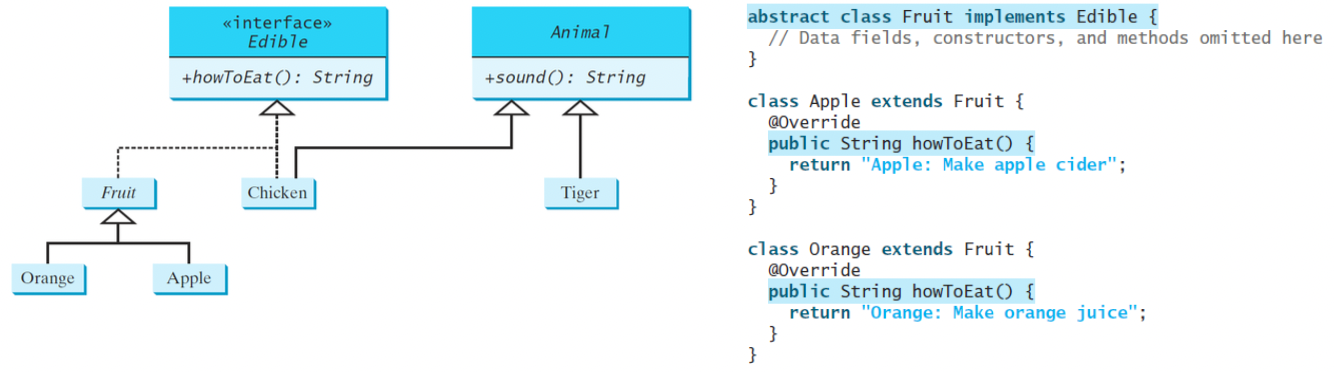
\includegraphics[scale=0.7]{Interface.png}
		\end{itemize}

	\item Generics
		\begin{itemize}
			\item Enable type parameterization
				\begin{itemize}
					\item Generic interfaces
					\item Generic classes
					\item Generic methods
				\end{itemize}
			\item Example: \textbf{ArrayList} class
				\begin{itemize}
					\item ArrayList$\langle$Integer$\rangle$ A = new ArrayList$\langle$Integer$\rangle$();
					\item ArrayList$\langle$String$\rangle$ B = new ArrayList$\langle$String$\rangle$();
				\end{itemize}
			\item Generic types must be reference types
			\item Enable error detection at compile time
			\item The \textbf{Comparable} interface
				\begin{itemize}
					\item Defines the \textbf{compareTo} method for comparing objects
					\item Defined as follows:\\[5pt]
\begin{minipage}{0.5\textwidth}
		\begin{Verbatim}
	public interface Comparable<T> {
		public int compareTo(T t);
	}
\end{Verbatim}
\end{minipage}
					\item The \textbf{compareTo} method determines the order of the calling object with \textbf{t} and returns a negative integer, zero, or a positive integer if the calling object is less than, equal to, or greater than \textbf{t}
					\item Many classes implement Comparable (e.g. \textbf{String}, \textbf{Integer})
				\end{itemize}
%			\newpage
			\item The \textbf{ArrayList} class
				\begin{itemize}
					\item Arrays can be used to store lists of objects. However, once an
					array is created, its size is fixed
					\item Java provides the generic class \textbf{ArrayList} whose size is variable
					\item Imported using: \textbf{import java.util.ArrayList;}
					\item Commonly used methods (\textbf{ArrayList<E>})
						\begin{itemize}
							\item \textbf{boolean add(E e)}
							\item \textbf{E get(int index)}
							\item \textbf{int size()}
							\item \textbf{boolean contains(Object o)}
							\item \textbf{int indexOf(Object o)}
						\end{itemize}
					\item An \textbf{ArrayList} could be traversed using a for-each loop
				\end{itemize}
			\newpage
			\item The \textbf{HashSet} class
				\begin{itemize}
					\item Generic class that can be used to store elements without duplicates
						\begin{itemize}
							\item No two elements e1 and e2 can be in the set such that e1.equals(e2) is true
						\end{itemize}
					\item Imported using: \textbf{import java.util.HashSet;}
					\item Objects added to the hash set should override \textbf{equals} and \textbf{hashCode} properly
					\item Commonly used methods (\textbf{HashSet$\langle$E$\rangle$})
						\begin{itemize}
							\item \textbf{boolean add(E e)}
							\item \textbf{int size()}
							\item \textbf{boolean contains(Object o)}
						\end{itemize}
					\item A \textbf{HashSet} could be traversed using a for-each loop
				\end{itemize}

			\item The \textbf{LinkedHashSet} class
				\begin{itemize}
					\item Elements of a \textbf{HashSet} are not necessarily stored in the same
					order they were added
					\item \textbf{LinkedHashSet} is a subclass of \textbf{HashSet} with a linked-list implementation that supports an ordering of the elements in the set
					\item Imported using: \textbf{import java.util.LinkedHashSet;}
				\end{itemize}
		\end{itemize}

	\item Exceptions
		\begin{itemize}
			\item Example\\
				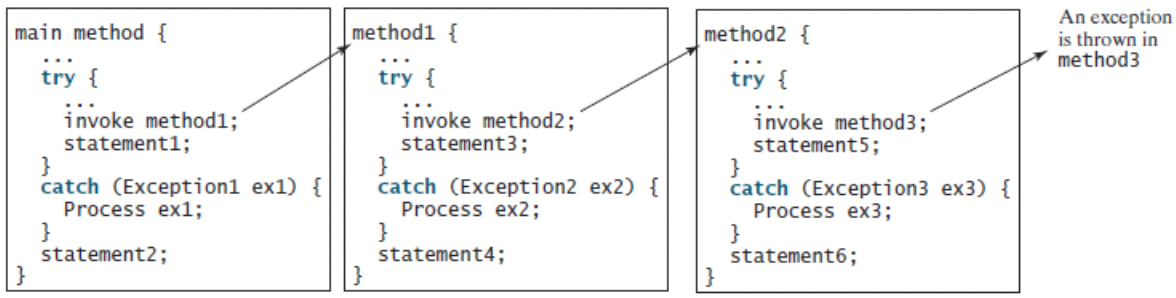
\includegraphics[scale=0.7]{Exceptions.png}
			\item Java has a \textbf{finally} clause that can be used to execute some code regardless of whether an exception occurs or is caught. For example:
				\begin{Verbatim}
				try {
					//statements;
				}
				catch Exception ex) {
					//handling ex; }
				finally {
					//final statements;
				}
				\end{Verbatim}
		\end{itemize}
\end{itemize}
	\newpage

\subsection*{Object Oriented Programming - Design Guidelines}
\begin{itemize}
	\item Methods Common to All Objects
		\begin{itemize}
			\item Always override hashCode when you override equals
			\item Always override toString
			\item ConsiderimplementingComparable
		\end{itemize}

	\item Classes and Interfaces
		\begin{itemize}
			\item Minimize accessibility
			\item Favor composition over inheritance
			\item Prefer interfaces to abstract classes
			\item Prefer lists to arrays
		\end{itemize}

	\item Methods
		\begin{itemize}
			\item Check parameters for validity
			\item Return empty arrays or collections, not \textbf{null}
			\item Document your API properly
		\end{itemize}

	\item Exceptions
		\begin{itemize}
			\item Use exceptions only for exceptional conditions
			\item Use checked exceptions for recoverable conditions and runtime exceptions for programming errors
			\item Do not ignore exceptions
		\end{itemize}

	\item General Programming (Naming Conventions)
		\begin{itemize}
			\item Package names should be hierarchical with the components separated by periods. Components should consist of lowercase alphabetic characters and, rarely, digits. e.g. \textbf{javax.swing.plaf.metal}
			\item Class and interface names should consist of one or more words, with the first letter of each word capitalized
			\item Method and field names follow the same typographical conventions as class and interface names, except that the first letter of a method or field name should be lowercase, for example, \textbf{ensureCapacity}
			\item The names of constant fields should consist of one or more uppercase words separated by the underscore character, for example, \textbf{NEGATIVE\textunderscore INFINITY}
			\item Local variable names have similar typographical naming conventions to member names, except that abbreviations are permitted, as are individual characters and short sequences of characters whose meaning depends on the context in which the local variable occurs, for example, \textbf{i}, \textbf{xref}
		\end{itemize}
\end{itemize}

\newpage

\section{Software Testing}
\begin{itemize}
	\item What is Software Testing?
		\begin{itemize}
			\item Running a program in order to find faults
				\begin{itemize}
					\item Examining the code without execution is \underline{not} testing
				\end{itemize}
			\item The main practical approach to validate/verify software
				\begin{itemize}
					\item Formal methods that aim at proving the correctness of a program are not
						scalable
				\end{itemize}
			\item “Program testing can be used to show the presence of bugs, but never to show their absence!” -- Edsger W. Dijkstra
		\end{itemize}
	\item Testing Levels
		\begin{itemize}
			\item Acceptance testing
				\begin{itemize}
					\item Test whether the software is acceptable to the user
				\end{itemize}
			\item System testing
				\begin{itemize}
					\item Test the overall functionality of the system
				\end{itemize}
			\item Integration testing
				\begin{itemize}
					\item Test how modules interact with each other
				\end{itemize}
			\item Module testing
				\begin{itemize}
					\item A module is a collection of related units the are assembled in a file, package, or class
					\item Test modules in isolation including how the components interact with each other
					\item \underline{Responsibility of the programmer}
				\end{itemize}
			\item Unit testing
				\begin{itemize}
					\item Test units (methods individually)
					\item \underline{Responsibility of the programmer}
				\end{itemize}
		\end{itemize}

	\item Black-Box and White-Box Testing
		\begin{itemize}
			\item Black-Box Testing
				\begin{itemize}
					\item Test are derived from external descriptions of the software
				\end{itemize}
			\item White-Box Testing
			\begin{itemize}
				\item Test are derived from source code internals of the software
				\item More expensive to apply
			\end{itemize}
		\end{itemize}

	\item Why is Software Testing Hard?
		\begin{itemize}
			\item Exhaustive testing is infeasible
				\begin{itemize}
					\item e.g. Exhaustively testing a method with two integer parameters would
					require $ \sim \negmedspace 10^{19} $ tests
				\end{itemize}
			\item Random/statistical testing is not effective
		\end{itemize}

	\item Why Do We Test Software?
		\begin{itemize}
			\item Software is everywhere
				\begin{itemize}
					\item Communication, transportation, healthcare, finance, education, etc.
				\end{itemize}
			\item Software failures could have severe consequences
				\begin{itemize}
					\item A 2002 NIST report estimated that defective software costs the U.S. economy \$59.5 billion per year and that improvements in testing could reduce this cost by about a third
					\item In certain areas such as healthcare and transportation, software failures could cost lives
				\end{itemize}
		\end{itemize}

	\item Infamous Software Failures
		\begin{itemize}
			\item Northeast blackout of 2003
				\begin{itemize}
					\item Caused by a failure of the alarm system
					\item Affected 40 million people in USA and 10 million people in Canada
					\item Contributed to at least 11 deaths
					\item Cost around \$6 billion
				\end{itemize}
			\item Ariane 5 explosion (1996)
				\begin{itemize}
					\item Unhandled floating point conversion exception
					\item Estimated loss: \$370 million
				\end{itemize}
			\item NASA’s Mars lander (1999)
				\begin{itemize}
					\item Crashed due to an integration fault
					\item Estimated loss: \$165 million
				\end{itemize}
			\item Boeing 737 Max
				\begin{itemize}
					\item Crashed due to overly aggressive software flight overrides
				\end{itemize}
			\item Boeing A220
				\begin{itemize}
					\item Engines failed after software update allowed excessive vibrations
				\end{itemize}
			\item Toyota brakes failure
				\begin{itemize}
					\item Dozens dead
					\item Thousands of crashes
				\end{itemize}
			\item Therac-25 radiation therapy machine
				\begin{itemize}
					\item Three patients were killedº
				\end{itemize}
		\end{itemize}

	\item Fault/Error/Failure
		\begin{itemize}
			\item \textbf{\textit{Software Fault}}: A static defect in the software
			\item \textbf{\textit{Software Error}}: An incorrect internal state that is the manifestation of
			some fault
			\item \textbf{\textit{Software Failure}}: External, incorrect behavior with respect to the requirements or another description of the expected behaviour
			\item The term \textbf{\textit{bug }}is often used informally to refer to all three of fault, error, and failure
				\begin{itemize}
					\item The first computer bug was an actual bug!
				\end{itemize}
			\item Example\\
				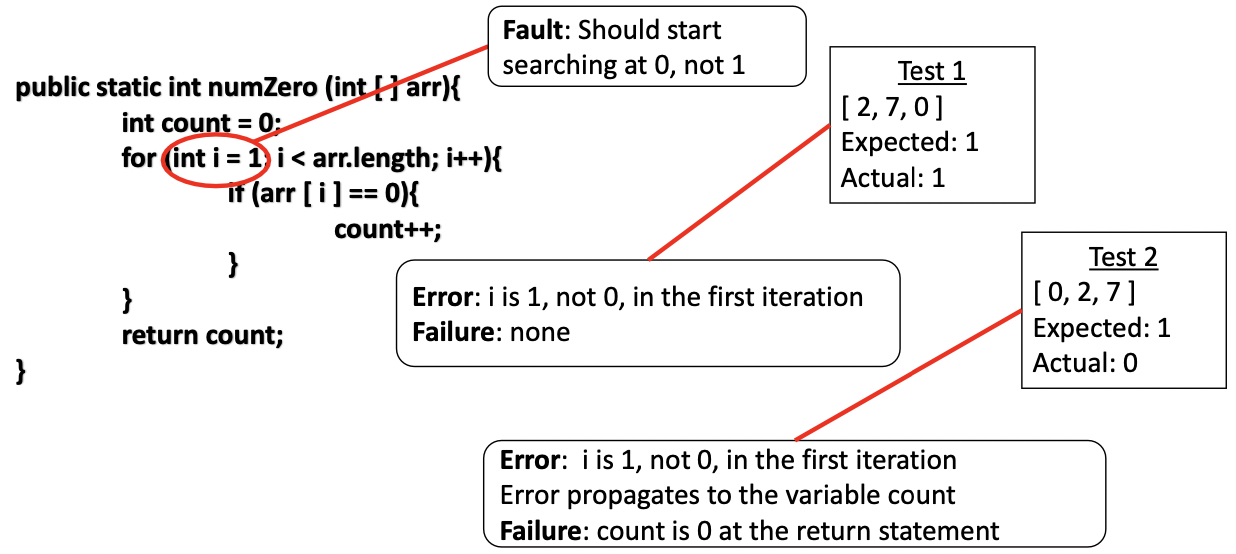
\includegraphics[scale=0.7]{FEF.png}
		\end{itemize}


	\item The RIPR model
		\begin{itemize}
			\item Four conditions are needed for a failure to be observed
				\begin{enumerate}
					\item \textbf{\textit{Reachability}}: a test must reach the location in the program that contains the fault
					\item \textbf{\textit{Infection}}: After the faulty location is executed, the state of the program must be incorrect
					\item \textbf{\textit{Propagation}}: The infected state must propagate through the rest of the execution and cause some output or final state of the program to be incorrect
					\item \textbf{\textit{Revealability}}: The tester must observe part of the incorrect portion of the final program state
				\end{enumerate}
				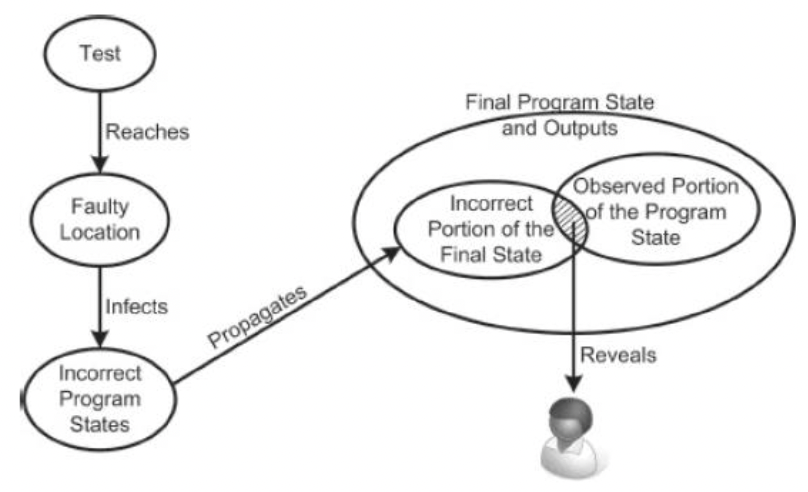
\includegraphics[scale=0.7]{RIPR.png}
		\end{itemize}

	\item Criteria-based Test Design
		\begin{itemize}
			\item \textbf{\textit{Coverage Criterion}}: A rule or collection of rules that impose test requirements on a test set
				\begin{itemize}
					\item e.g. For each statement in the code, there should be at least one test case that covers it
				\end{itemize}
			\item Coverage criteria give us structured, practical ways to search the input space. Satisfying a coverage criterion gives a tester some amount of confidence in two crucial goals:
				\begin{enumerate}
					\item We have looked in many corners of the input space, and
					\item Our tests have a fairly low amount of overlap
				\end{enumerate}
			\item Criteria subsumption
				\begin{itemize}
					\item $ C_1 $ subsumes $ C_2 $ if and only if every test set that satisfies $ C_1 $ satisfies $ C_2 $
				\end{itemize}
		\end{itemize}

	\item Graph Coverage
		\begin{itemize}
			\item The software is modeled as a graph where nodes and edges could represent:
				\begin{itemize}
					\item Methods and calls
					\item Statements and branches
					\item Etc.
				\end{itemize}
			\item Coverage criteria are defined based on the graph. For example:
				\begin{itemize}
					\item Cover every node
					\item Cover every edge
					\item Cover every path
					\item Etc.
				\end{itemize}


			\item Example (Control Flow Graph)\\
				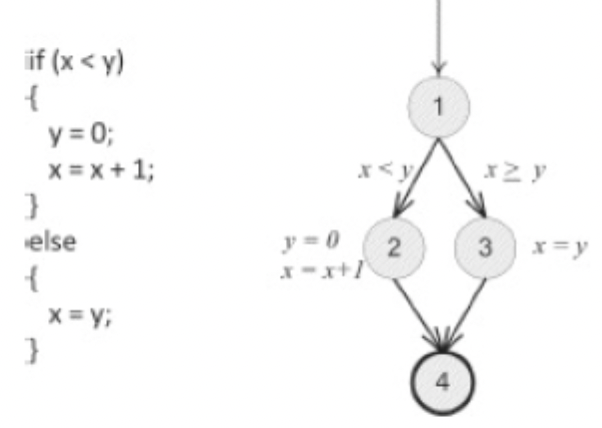
\includegraphics[scale=0.7]{CFG.png}
		\end{itemize}

	\item Logic Coverage
		\begin{itemize}
			\item Involves the boolean expressions of the code
			\item Coverage criteria include:
				\begin{itemize}
					\item Predicate coverage
					\item Clause coverage
					\item Combinational coverage
					\item Etc.
				\end{itemize}
			\item Example
\begin{Verbatim}
	if(((a>b) || c) && (x<y))
		...
	else
		...
\end{Verbatim}
			\item Predicate coverage
				\begin{itemize}
					\item The test set should make each predicate evaluate to true and false
					\item e.g. $ ((a>b) \, || \, c) \, \&\& \, (x<y) = \{\text{True}, \text{False}\} $
				\end{itemize}
			\item Clause coverage
				\begin{itemize}
					\item The test set should make each clause evaluate to true and false
					\item e.g. $ (a>b) = \{\text{True}, \text{False}\}, c = \{\text{True}, \text{False}\}, (x<y) = \{\text{True}, \text{False}\} $
				\end{itemize}
		\end{itemize}

	\item Active clause coverage
		\begin{itemize}
			\item Clause coverage has a weakness
				\begin{itemize}
					\item The values do not always make a difference
				\end{itemize}
			\item A clause $ c_i$ in predicate $ p $, called the major clause, determines $ p $ \textit{if and only if} the values of the remaining minor clauses $ c_j $ are such that changing $ c_i $ changes the value of $ p $
			\item Two requirements for each $ c_i $: $ c_i $ evaluates to true and $ c_i $ evaluates to false
			\item This is a form of MCDC, which is required by the FAA for safety critical
			software

		\end{itemize}

	\item Inactive clause coverage
		\begin{itemize}
			\item Ensures that “major” clauses do not affect the predicates
			\item Four requirements for each $ c_i $
				\begin{enumerate}
					\item $c_i$ evaluates to true with p true
					\item $c_i$ evaluates to false with p true
					\item $c_i$ evaluates to true with p false
					\item $c_i$ evaluates to false with p false
				\end{enumerate}
			\item Example
				\begin{itemize}
					\item Testing the control software for a shutdown system in a reactor where the specification states that the status of a particular valve (\textbf{open} vs. \textbf{closed}) is relevant to the reset operation in \textbf{Normal} mode, but not in \textbf{Override} mode
				\end{itemize}
		\end{itemize}

	\item Test Oracles
		\begin{itemize}
			\item A \textit{test oracle} is an encoding of the expected results of a given test
				\begin{itemize}
					\item e.g. JUnit assertion
				\end{itemize}
			\item Must strike a balance between checking too much (unnecessary cost) and checking too little (perhaps not revealing failures)
			\item What should be checked?
				\begin{itemize}
					\item The output state is everything that is produced by the software under test, including outputs to the screen, file, databases, messages, and signals
					\item Each test should have a goal and testers should check the output(s) that are mainly related to that goal
						\begin{itemize}
							\item At the unit testing level, checking the return values of the methods and returned parameter values are almost always enough
							\item At the system level, it is usually sufficient to check the directly visible output such as to the screen
						\end{itemize}
				\end{itemize}

			\item How to determine what the correct results are
			\begin{itemize}
				\item Specification-Based direct verification of outputs
				\begin{itemize}
					\item e.g. “a \textbf{sort} program should produce a permutation of its input in increasing order ”
					\item Specifications are hard to write
				\end{itemize}
			\item Redundant computations
				\begin{itemize}
					\item Refer to another trustworthy implementation of the program
					\item Usually used for regression testing
				\end{itemize}
			\item Consistency checks
				\begin{itemize}
					\item Check whether certain properties hold (e.g. a value representing probability
					should neither be negative nor larger than one)
				\end{itemize}
			\end{itemize}
		\end{itemize}
\end{itemize}

\newpage

\section{Design Patterns}
\begin{itemize}
	\item What are Design Patterns
		\begin{itemize}
			\item Descriptions of communicating objects and classes that are customized to \textbf{\underline{solve}} a general design \textbf{\underline{problem}} in a particular \textbf{\underline{context}}
			\item 	Gamma et al. described 23 design patterns divided into three categories:
				\begin{enumerate}
					\item Creational patterns
					\item Structural patterns
					\item Behavioral patterns
				\end{enumerate}
		\end{itemize}

	\item Creational Patterns
		\begin{itemize}
			\item Concern the process of object creation
			\item Six creational patterns\\[-10pt]
				\begin{minipage}[t]{0.25\textwidth}
					\begin{enumerate}
						\item Factory Method
						\item Abstract Factory
						\item Singleton
					\end{enumerate}
				\end{minipage}
				\begin{minipage}[t]{0.4\textwidth}
					\begin{enumerate}
						\setcounter{enumi}{3}
						\item Prototype
						\item Builder
						\item Object Pool
					\end{enumerate}
				\end{minipage}
		\end{itemize}

	\item Structural Patterns
		\begin{itemize}
			\item Deal with the composition of classes or objects
			\item Seven structural patterns\\[-10pt]
				\begin{minipage}[t]{0.25\textwidth}
					\begin{enumerate}
						\item Adapter
						\item Bridge
						\item Composite
						\item Decorator
					\end{enumerate}
				\end{minipage}
				\begin{minipage}[t]{0.4\textwidth}
					\begin{enumerate}
						\setcounter{enumi}{4}
						\item Facade
						\item Flyweight
						\item Proxy
					\end{enumerate}
				\end{minipage}
		\end{itemize}

	\item Behavioral Patterns
		\begin{itemize}
			\item Characterize the ways in which classes or objects interact and distribute responsibility
			\item Ten Behavioral patterns\\[-10pt]
			\begin{minipage}[t]{0.4\textwidth}
				\begin{enumerate}
					\item Chain of Responsibility
					\item Command
					\item Interpreter
					\item Iterator
					\item Mediator
				\end{enumerate}
			\end{minipage}
			\begin{minipage}[t]{0.4\textwidth}
				\begin{enumerate}
					\setcounter{enumi}{5}
					\item Memento
					\item Observer
					\item State
					\item Strategy
					\item Template
				\end{enumerate}
			\end{minipage}
		\end{itemize}

	\item Singleton (Creational)
		\begin{itemize}
			\item Intent: Ensure a class has only one instance, and provide a global point of access to it\\
			\begin{center}
				\begin{tabular}{| l |}
				\hline
				Singleton\\
				\hline
				$ - $instance: Singleton\\
				\hline
				$ - $Singleton()\\
				+getInstance(): Singleton\\
				\ldots\\
				\hline
			\end{tabular}	\textit{	( $ - $ means private, $ + $ means public)}
			\end{center}
		\end{itemize}
%
	\item Facade (Structural)
		\begin{itemize}
			\item Intent: Hide complexities and provide a unified interface to a set of interfaces in a subsystem\\[-10pt]
				\begin{center}
					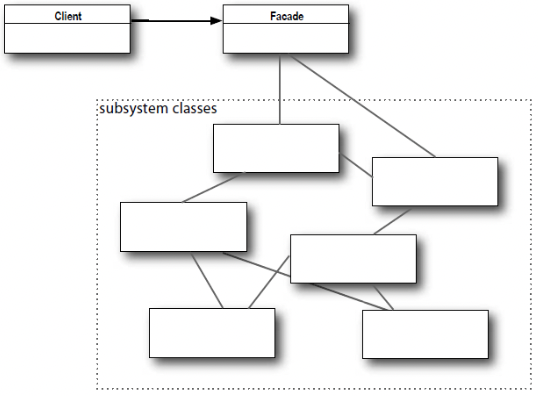
\includegraphics[scale=0.8]{Facad.png}
				\end{center}
		\end{itemize}
	\newpage
	\item Adapter (Structural)
		\begin{itemize}
			\item Intent: Let classes work together that couldn't otherwise because of incompatible interfaces\\[-10pt]
				\begin{center}
					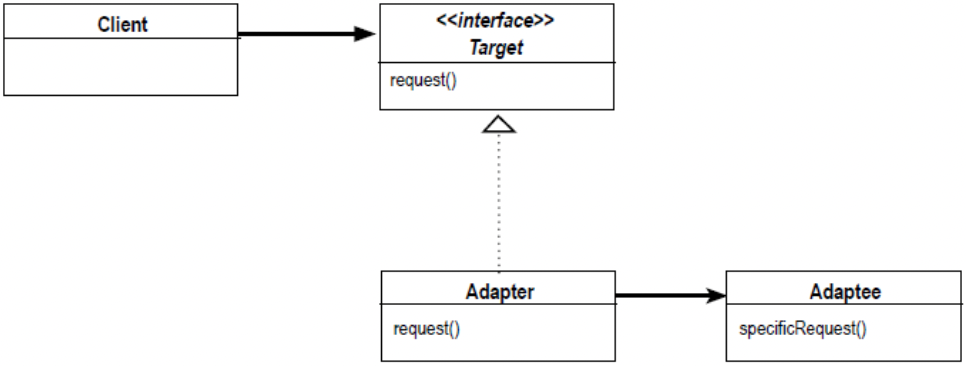
\includegraphics[scale=0.7]{Adapter.png}
				\end{center}
		\end{itemize}

	\item Observer (Behavioral)
		\begin{itemize}
			\item Intent: Define a one-to-many dependency between objects so that when one object changes state, all its dependents are notified and updated automatically\\[-10pt]
				\begin{center}
					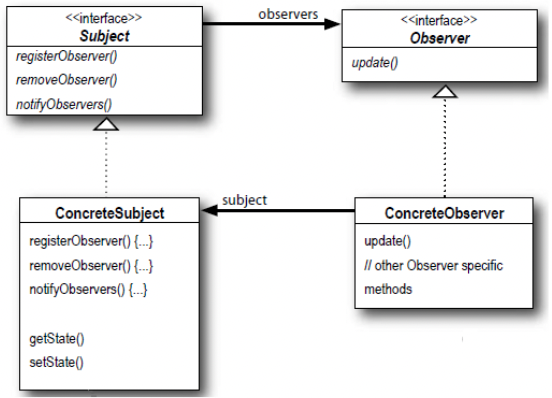
\includegraphics[scale=0.9]{Observer.png}
				\end{center}
		\end{itemize}
%	\newpage
	\item Strategy (Behavioral)
		\begin{itemize}
			\item Intent: Define a family of algorithms, encapsulate each one, and make them interchangeable\\[-10pt]
			\begin{center}
				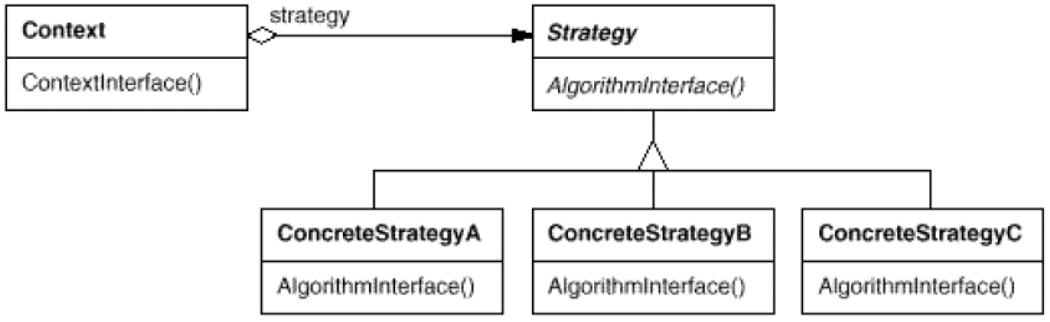
\includegraphics[scale=0.8]{Strategy.png}
			\end{center}
		\end{itemize}
\end{itemize}
\end{document}

